\chapter{Logistyka i łańcuchy dostaw}
\label{c2:c2}

\section{Logistyka jako dziedzina wiedzy}
	\subsection{Wiedza a nauka}	
		\begin{quote}
			\textit{
				``Pojęcie wiedzy jest bowiem pojęciem szerszym od nauki,
				obejmuje bowiem wszelkie i na każdej drodze zdobyte wiadomości
				tak teoretyczne, jak i praktyczne \cite{organizacja_badan_ocen_prac_naukowych}.''
			}
		\end{quote}
		
		Gdzie jednak leży granica ? Wiedzę najłatwiej opisać jako środek, pomagający 
		nam zdobywać kolejne szczyty w sposób coraz lepszy i efektywny. Nauka, z drugiej strony,
		daje potężny oręż pomagający, jednocześnie, odkrywać nowe problemy i je rozwiązywać.
		
	\subsection{Logistyka i wojskowe korzenie}
		Logistyka znana, i co ważniejsze stosowana, była już w czasach starożytnych, gdzie jednoznacznie
		była utożsamiana z zaopatrzeniem oddziałów wojskowych w żywność, broń oraz odpowiedni
		sprzęt potrzebny do prowadzenia działań wojennych. Geneza słowa pochodzi od greckich
		słów \emph{logos} lub \emph{logicos} odnoszących się do syntezy dziedziny jaką jest logistyka,
		czyli do kalkulacji oraz wykorzystania rozumu i rozsądku. To, czym dzisiaj zajmują się planiści w 
		firmach produkcyjnych - \emph{zarządzanie wielkimi organizacjami, dużej dynamice zmian} - było kiedyś 
		domeną strategów wojskowych. Z każdym krokiem, gdzie historia posuwała
		się naprzód, logistyka zmieniała się i różnicowała. Niemniej pierwotny cel pozostał ten sam - 
		\emph{dostarczyć siłom wojskowym wszystkiego, co niezbędne do prowadzenia walk} \\
		
		Szczególnie bujny rozwój to lata II wojny światowej oraz podwaliny logistyki współczesnej
		podłożone przez amerykańskich strategów, starających się rozwiązywać problemy zaopatrzenia
		armii amerykańskiej na frontach Europy oraz obszarów objętych działaniami wojennymi wojny pacyficznej. 
		\cite{logistyka_w_przedsiebiorstwie}\cite{logistyka_jako_dziedzina_wiedzy_cz1}.
		
	\subsection{Logistyka współcześnie znana jako wynik zmian na rynku}
		\begin{figure}[h]
			\centering
			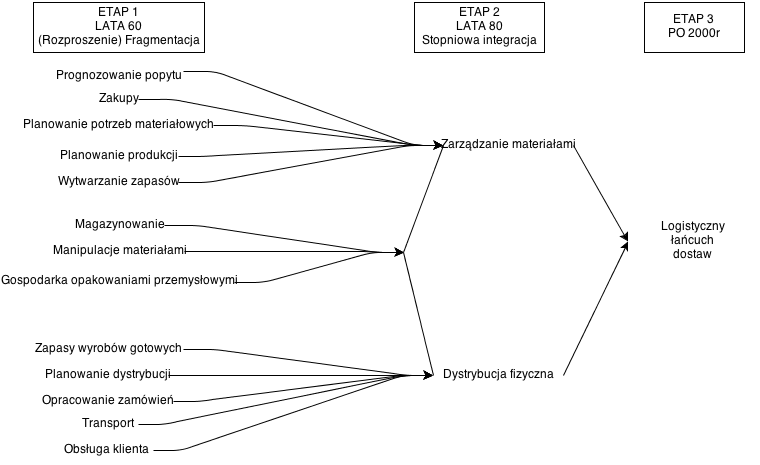
\includegraphics[width=\textwidth]{images/etapy_rozwoju_logistyki}
			\caption[3 etapy rozwoju logistyki]{
				3 Etapy rozwoju logistyki \\
				źródło: \cite{logityka_w_przedsiebiorstwie_sarsjusz_wolski_skowronek}
			}
		\end{figure}
		To co jest dzisiaj obserwujemy i to co tak chętnie nazywane jest logistyką, 
		można bardzo łatwo zdefiniować jako reakcję na popyt od
		strony przedsiębiorstw (produkcyjnych, handlowych itp.) na coraz trudniejsze warunki na
		rynku: \textbf{konkurencję, rosnące wymagania odbiorców, wzrost kosztów, kryzys ekonomiczny}.
		Wspomniane firmy poszukują więc wszelkich metod optymalizacji swojej działalności, 
		które mogą zostać zaimplementowane w zgodzie z aktualnym stanem otoczenia firmy.\\
		
		Logistyka zaczęła więc obejmować swoim zasięgiem coraz więcej obszarów funkcjonalnych, które
		wymagały zracjonalizowania i zoptymalizowania, aby stać się źródłem wysokiej wartości dodanej, do której
		dąży się poprzez odpowiednie \emph{zarządzanie} \cite{logistyka_jako_dziedzina_wiedzy_cz1}.		
		
		\paragraph{Dziedzina interdyscyplinarna} jest prawdopodobnie najlepszym zwrotem, 
		który mógłby opisać wynik tych transformacji i oddziaływań na ciągle ewoluujący organizm, swoim
		zasięgiem obejmującym szeroki wachlarz innych działań człowieka. Począwszy od momentu złożenia
		zamówienia przez klienta po odebranie przez niego gotowego produktu, to właśnie logistyka jest
		tym, co czuwa nad mnogością procesów przeplatających się po drodze \cite{logistyka_jako_dziedzina_wiedzy_cz2}.	
		
	\subsection{Logistic management - Zarządzania logistyczne}
		\begin{quote}
			\textit{
				``\emph{Zarządzanie logistyczne} - jest funkcją integrującą, której głównym zadaniem jest
				koordynacja i jednoczesna optymalizacja działań firmy na wszystkich poziomach
				\footnote{strategicznym, operacyjnym oraz taktycznym}. Ponadto zadaniem \emph{zarządzania logistycznego} jest
				integracja czynności logistycznych z elementami marketingu, dystrybucji, finansów oraz technologii
				informatycznych \cite{csmp_logistic_management}.''
			}
		\end{quote}
		
		Bazując na powyższej definicji zarządzanie logistyczne uwzględnia także czynności takie jak:
		obsługa transportu, floty, magazynów, gospodarki materiałowej, obsługi zamówień, 
		projektowanie sieci powiązań, ewidencja sprzętu,
		planowanie dostaw oraz przewidywanie zapotrzebowania oraz korzystanie z 
		usług outsourcingowych firm trzecich. Jednocześnie działając na wielu poziomach, 
		funkcje logistyczne często uwzględniają zaopatrzenie, planowanie produkcji, harmonogramowanie, 
		pakowanie, komplementacje oraz obsługę klienta. Wszystkie właśnie wymienione czynności
		objawiają się na wszystkich poziomach planowania oraz działalności - taktycznym, operacyjnym oraz
		strategicznym \cite{csmp_logistic_management}.

\section{Logistyka w działaniu przedsiębiorstwa}  
	W ramach przedsiębiorstw logistyka jest zbiorem konkretnych procesów, 
	gdzie każdy z nich odpowiada pewnemu rozwiązaniu organizacyjnemu i przynależy do konkretnego 
	elementu strukturalnego danej instytucji. W połączeniu z otoczeniem, w którym wyróżnia się:
	\begin{itemize}
		\item \textbf{mikrootoczenie} - do którego przedsiębiorstwo musi się dostosować,
		\item \textbf{makrootoczenie} - na które przedsiębiorstwo ma bezpośredni wpływ i w którym działa.
	\end{itemize}
	danego przedsiębiorstwa, wspomniane wcześniej procesy, tworzą \textbf{system logistyczny}, który określa
	\begin{itemize}
		\item zasady, reguły według których należy realizować procesy;
		\item zbiór środków, potrzebnych do ich realizacji.
	\end{itemize}
	Warto w tym miejscu wprowadzić kolejne trzy intuicyjne pojęcia. Podobnie jak na rynku
	działają firmy o zasięgu globalnym i lokalnym oraz mali dostawcy, którzy sprzedają
	owoce swojej pracy na lokalnym targu, a także dostawcy obejmujący swym zasięgiem dużą ilości
	odbiorców lokalnych, tak i w odniesieniu do \textbf{systemów logistycznych}
	istnieje podobny podział. Wyróżnia się bowiem systemy:
	\begin{itemize}
		\item[*] mikrologistyczne 	- będące w istocie pojedynczymi podmiotami gospodarki (firmami produkcyjnymi, itp.),
		\item[*] makrologistyczne 	- będące synonimem gospodarki jako tworu jednostkowego,
		\item[*] metalogistyczne	- będące grupami powiązanych ze sobą systemów mikrologistycznych, 
		czyli \textbf{łańcuchy dostaw}\cite{systemy_logistyczne_podstawy_funkcjonowania}.
	\end{itemize}

\section{Łańcuchy dostaw}
\label{c2:supply_chains}
	W dzisiejszych czasach patrzy się na logistykę 
	głównie przez pryzmat łańcucha dostaw jako
	elementu, łączącego w sobie takie składowe przedsiębiorstw jak:
	\begin{enumerate}
		\item zaopatrzenie,
		\item magazynowanie,
		\item dystrybucje,
		\item zwroty,
		\item utylizacje.
	\end{enumerate}
	
	W każdym z tych etapów niezmiennie najważniejsza 
	pozostaje \textbf{informacja}, której wartość najłatwiej
	opisać, jako równoważną wymiernym wynikom finansowym. 
	Na drugim miejscu paradoksalnie pozostaje przepływ
	samych towarów, materiałów czy też produktów. 
	Bowiem sam w sobie, nie daje on tego, co pozwala
	firmie reagować na zmiany w swoim otoczeniu.
	
	\subsection{Ewolucja tradycyjnych łańcuchów dostaw}
		\hspace{15pt}Łańcuchy dostaw podobne do przedstawionego na rysunku \ref{fig:simple_supply_chain} już dzisiaj 
		zaczynają być utożsamiane z przestarzałymi, chociaż
		wciąż dobrze sprawdzają się w mniejszych przedsiębiorstwach. 
		Niemniej te większe stawiają na ideę ciągłego doskonalenia
		i skracają swoje łańcuchy dostaw poprzez integrowanie 
		systemów poszczególnych jego uczestników.
		Integracja ta daje pewną niezaprzeczalną zaletę jaką jest ułatwienie 
		długoterminowej współpracy, wspólne podejmowanie decyzji, czy też
		dzielenie ryzyka. Rezultatem tego długoterminowego
		podejścia jest zwiększona konkurencyjność na rynku \cite{zarzadzanie_lancuchem_dostaw_w_dobie_gospodarki_elektroniczej}.\\
		
		\begin{figure}[h]
			\centering
			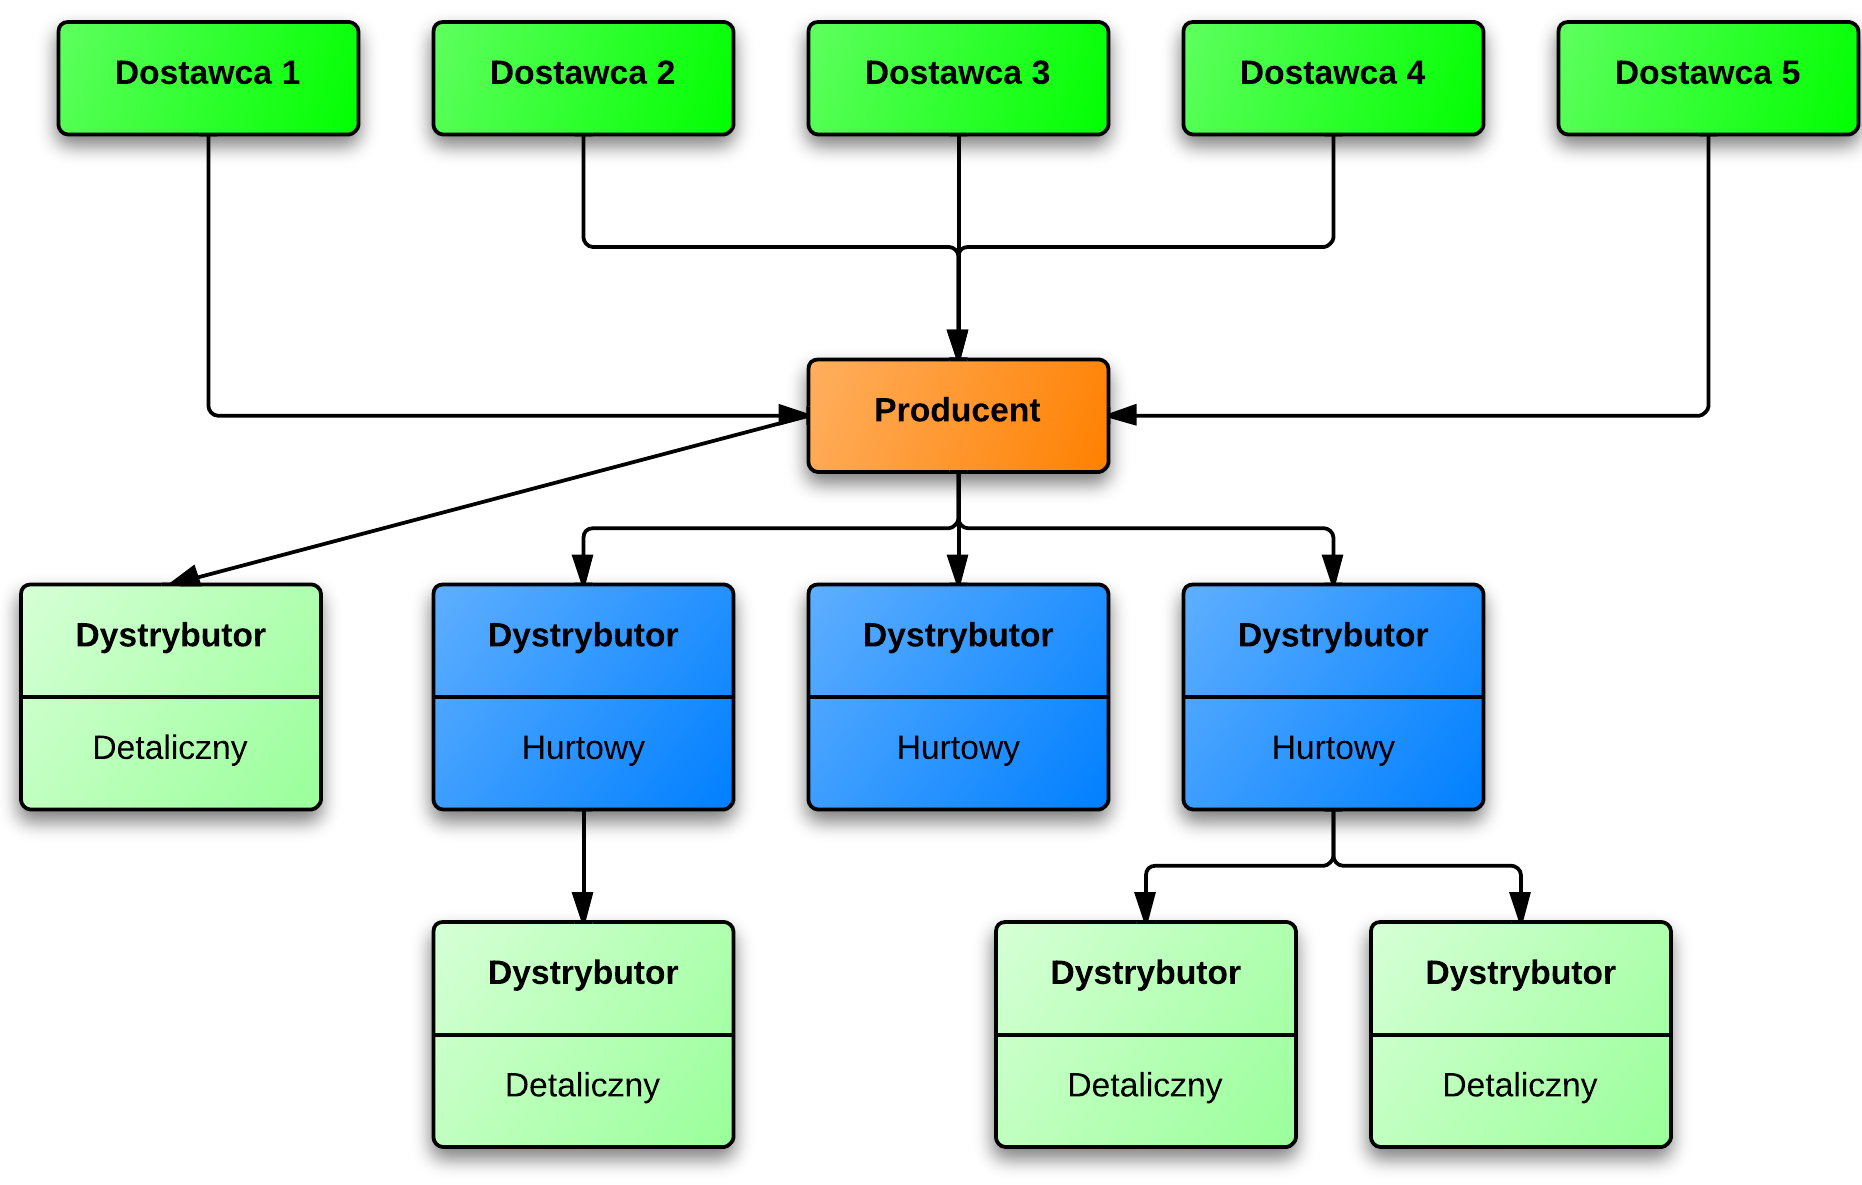
\includegraphics[width=370px, height=300px]{images/BasicSupplyChain}
			\caption[Schemat budowy prostego łańcucha dostaw]{
				Tradycyjny łańcuch dostaw \\
				źródło: opracowanie własne na podstawie \cite{zarzadzanie_lancuchem_dostaw_w_dobie_gospodarki_elektroniczej}
			}
			\label{fig:simple_supply_chain}
		\end{figure}		
		
		W momencie kiedy klient oczekuje dostawy nieuszkodzonego 
		towaru najwyżej jakości w ciągu 24h sprawne zarządzanie 
		łańcuchem dostaw wydaje się niezbędne. Samo jego znaczenie staje
		się tym wyrazistsze dla walki o klientów, jeśli sami zainteresowani
		zdają sobie z tego sprawę. Ponadto na dzisiejszym rynku nie liczy się
		już tak bardzo kto, a jak szybko i za jaką cenę.
		
	\subsection{Zarządzanie łańcuchem dostaw}
		\begin{figure}[h]
			\centering
			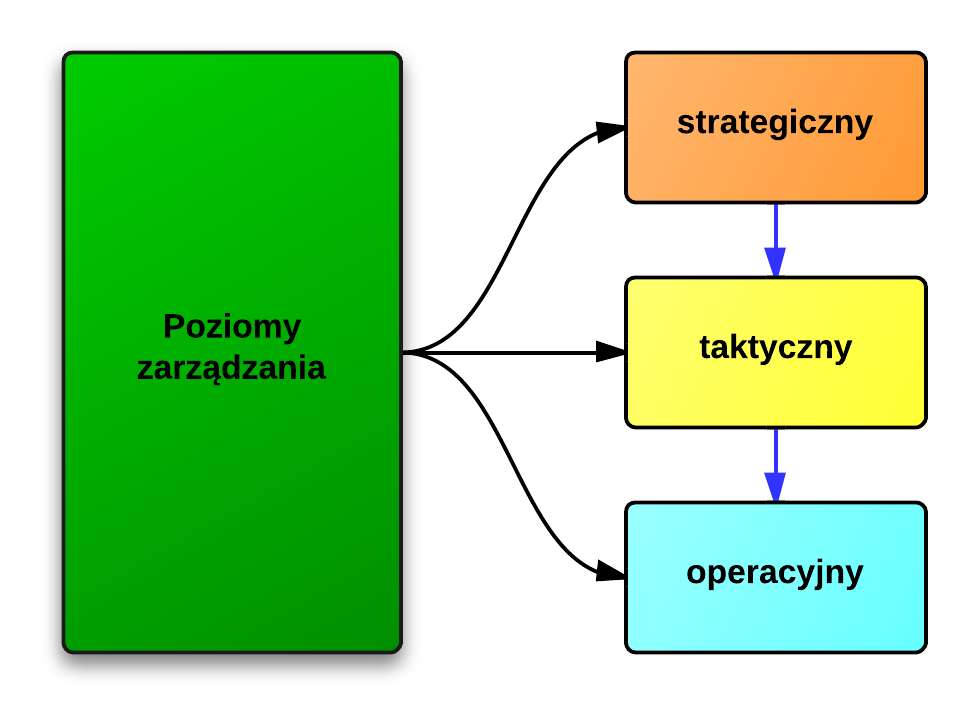
\includegraphics[width=0.8\textwidth]{images/3LevelsScm}
			\caption[3 poziomy zarządzania łańcuchem dostaw]{
				3 poziomy zarządzania\\
				źródło: opracowanie własne na podstawie \cite{ewolucja_lancuchow_dostaw_cz1}
			}
			\label{fig:3_levels_of_supply_chain}
		\end{figure}
		
		Wzrost kompleksowości i zakresu procesów, jakie wyróżnić można
		w łańcuchach dostaw, rośnie i bardzo możliwe, że taka tendencja będzie
		się wciąż utrzymywać. Przyczyną takiego stanu rzeczy jest rynek zbytu
		i zaopatrzenie oficjalnie nieograniczony dzięki globalnemu zasięgowi
		sieci Internet i możliwości transportu z lub do odległych rejonów kontynentu.
		Także sam produkt nie pozostaje bez znaczenie, jak i zmiana specyfikacji kontaktów
		i interakcji zachodzących miedzy uczestnikami łańcucha dostaw.
		
		Łańcuch dostaw zarządzany jest, podobnie jak przedsiębiorstwo, na 3 różnych poziomach:
		\begin{itemize}
			\item \textbf{Poziom strategiczny} 	- jego zadaniem jest globalne,
			w pojęciu relatywnym, odnoszącym się do łańcucha dostaw, kształtowanie oraz optymalizacja
			łańcucha dostaw;
			\item \textbf{Poziom taktyczny}		- obejmuje swoim zasięgiem operacje planowania wszelkich działań, 
			których	wyniki są niezbędne do zapewnienie prawidłowej pracy przedsiębiorstwa. Można tutaj wyróżnić 
			chociażby operacje:
			\begin{enumerate}
				\item planowania produkcji,
				\item zarządzania dostawcami,
				\item zarządzanie popytem,
				\item planowanie transportu;
			\end{enumerate}
			\item \textbf{Poziom operacyjny} 	- są to operacje faktycznego działania, obejmujące swoim zasięgiem
			wykonywanie ustaleń dokonanych na \emph{poziomie taktycznym} \cite{ewolucja_lancuchow_dostaw_cz1}.
		\end{itemize}